\documentclass[a4paper,12pt]{article}

%%% Работа с русским языком
\usepackage{cmap}					% поиск в PDF
\usepackage{mathtext} 				% русские буквы в формулах
\usepackage[T2A]{fontenc}			% кодировка
\usepackage[utf8]{inputenc}			% кодировка исходного текста
\usepackage[english,russian]{babel}	% локализация и переносы
\usepackage{xcolor}
\usepackage{hyperref}
 % Цвета для гиперссылок
\definecolor{linkcolor}{HTML}{00FFFF} % цвет ссылок
\definecolor{urlcolor}{HTML}{4682B4} % цвет гиперссылок

\hypersetup{pdfstartview=FitH,  linkcolor=linkcolor,urlcolor=urlcolor, colorlinks=true}

%%% Дополнительная работа с математикой
\usepackage{amsfonts,amssymb,amsthm,mathtools} % AMS
\usepackage{amsmath}
\usepackage{icomma} % "Умная" запятая: $0,2$ --- число, $0, 2$ --- перечисление

%% Номера формул
%\mathtoolsset{showonlyrefs=true} % Показывать номера только у тех формул, на которые есть \eqref{} в тексте.

%% Шрифты
\usepackage{euscript}	 % Шрифт Евклид
\usepackage{mathrsfs} % Красивый матшрифт

%% Свои команды
\DeclareMathOperator{\sgn}{\mathop{sgn}}

\usepackage{enumerate}
%% Перенос знаков в формулах (по Львовскому)
\newcommand*{\hm}[1]{#1\nobreak\discretionary{}
{\hbox{$\mathsurround=0pt #1$}}{}}
% графика
\usepackage{graphicx}
\graphicspath{{pictures/}}
\DeclareGraphicsExtensions{.pdf,.png,.jpg}
\author{Бурмаzшев Григорий, 208. \href{https://teleg.run/burmashev}{@burmashev}}
\title{Дискретная математика. Коллок -- 1. Определения и задачи по ним.}

\begin{document}
{\Large \begin{center}
Бурмашев Григорий.  208. Матан -- 3
\end{center}}
\begin{center}

\includegraphics[scale=1]{pivo.png}
\end{center}
\begin{center}
{\Huge \textbf{ТЕБЕ}}
\end{center}

\newpage
\section*{Номер 10}
\subsection*{a)}
\[
f(x) = (x+1)(x-2)^2
\]
Проведем исследование функции и построим её график.
\begin{enumerate}
\item \textbf{Область определения и поведение функции на границах:}

Функция определена всюду.

\[
\lim_{x \rightarrow \infty} f(x) = \infty
\]
\[
\lim_{x \rightarrow -\infty}  f(x) = -\infty
\]
\item \textbf{Нули и знаки функции:}
\[
(x+1)(x-2)^2 = 0
\]
\[
x = -1; x = 2
\]
\item \textbf{Экстремумы и монотонность:}
\[
f'(x) = 1 \cdot (x-2)^2 + (x+1) \cdot 2(x-2) = 3x(x-2)
\]
\[
f'(x) = 0 : \; x = 2; x = 0
\]
\[
f(2) = 0; f(0) = 4
\]
\begin{center}
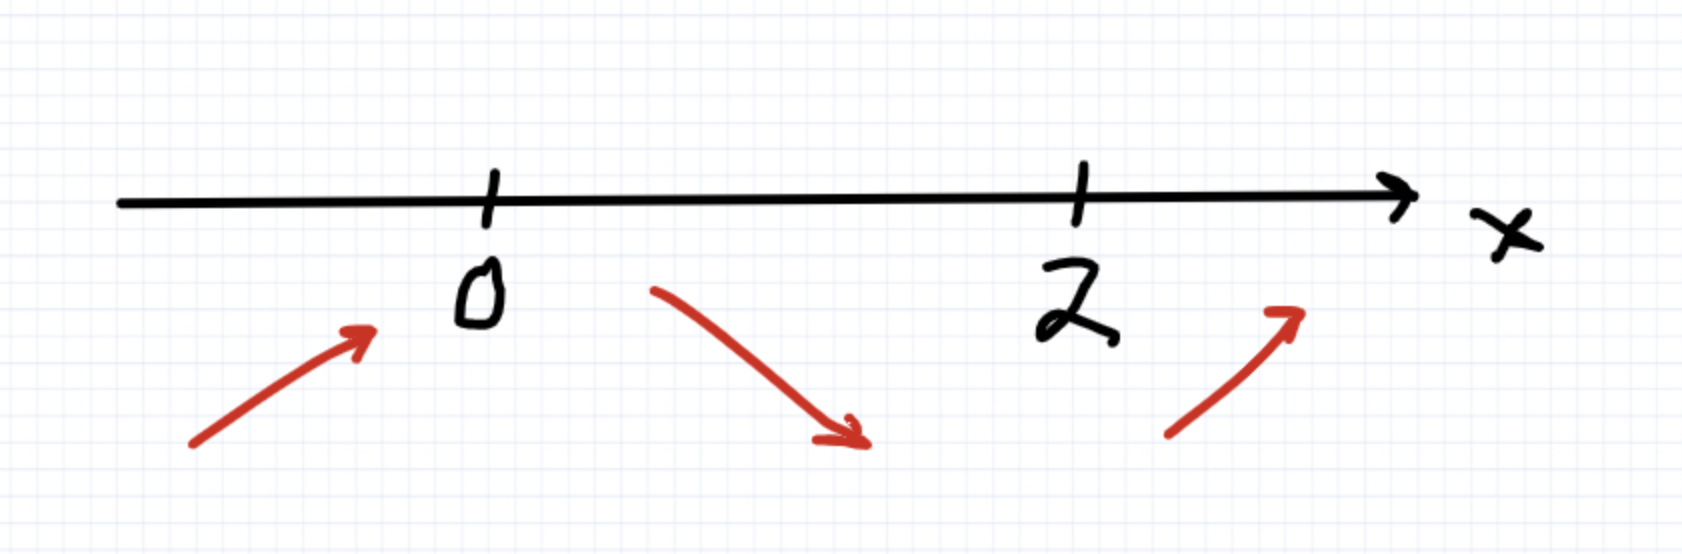
\includegraphics[scale=0.2]{1.png}
\end{center}
\newpage
\item \textbf{Выпуклость:}
\[
f''(x) = 6(x-1)
\]
\[
f''(x) = 0 : \; x = 1
\]
\[
f(1) = 2
\]
\begin{center}
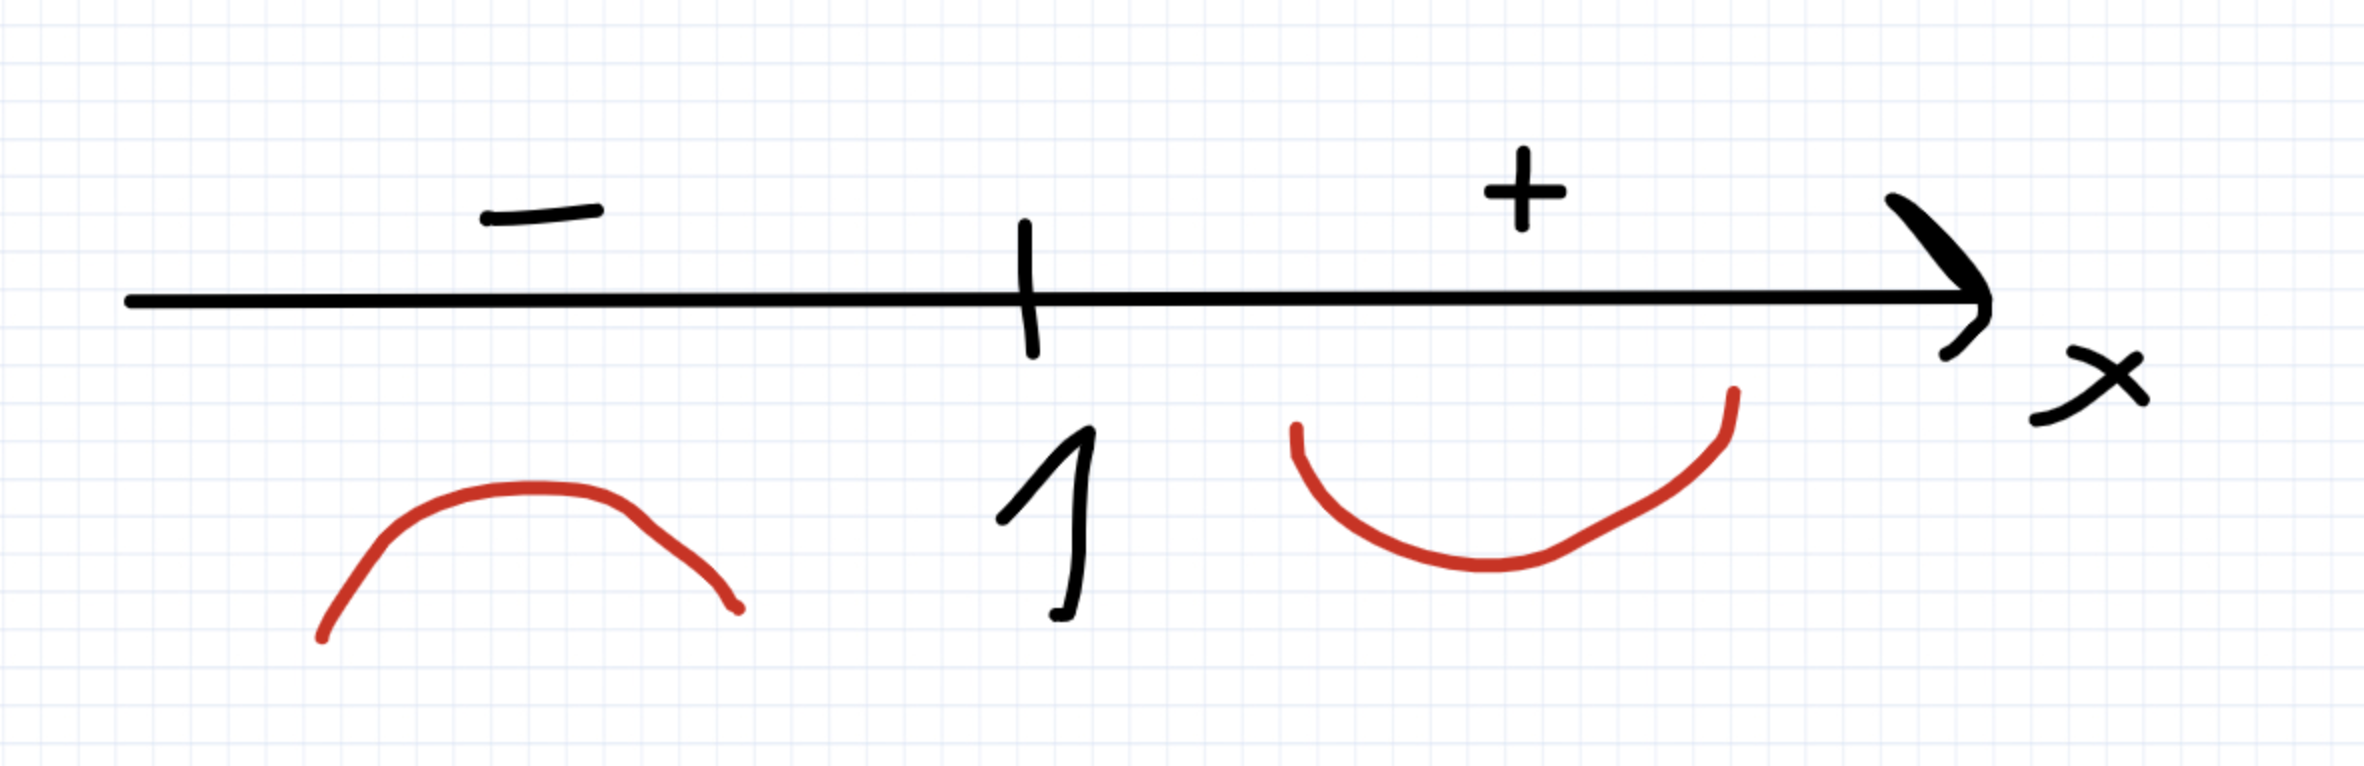
\includegraphics[scale=0.15]{2.png}
\end{center}
\item \textbf{Ассимптоты:}
\[
k = \lim_{x \rightarrow \infty} \frac{(x+1)(x-2)^2}{x} = \infty 
\]
\item \textbf{График:}
\begin{center}
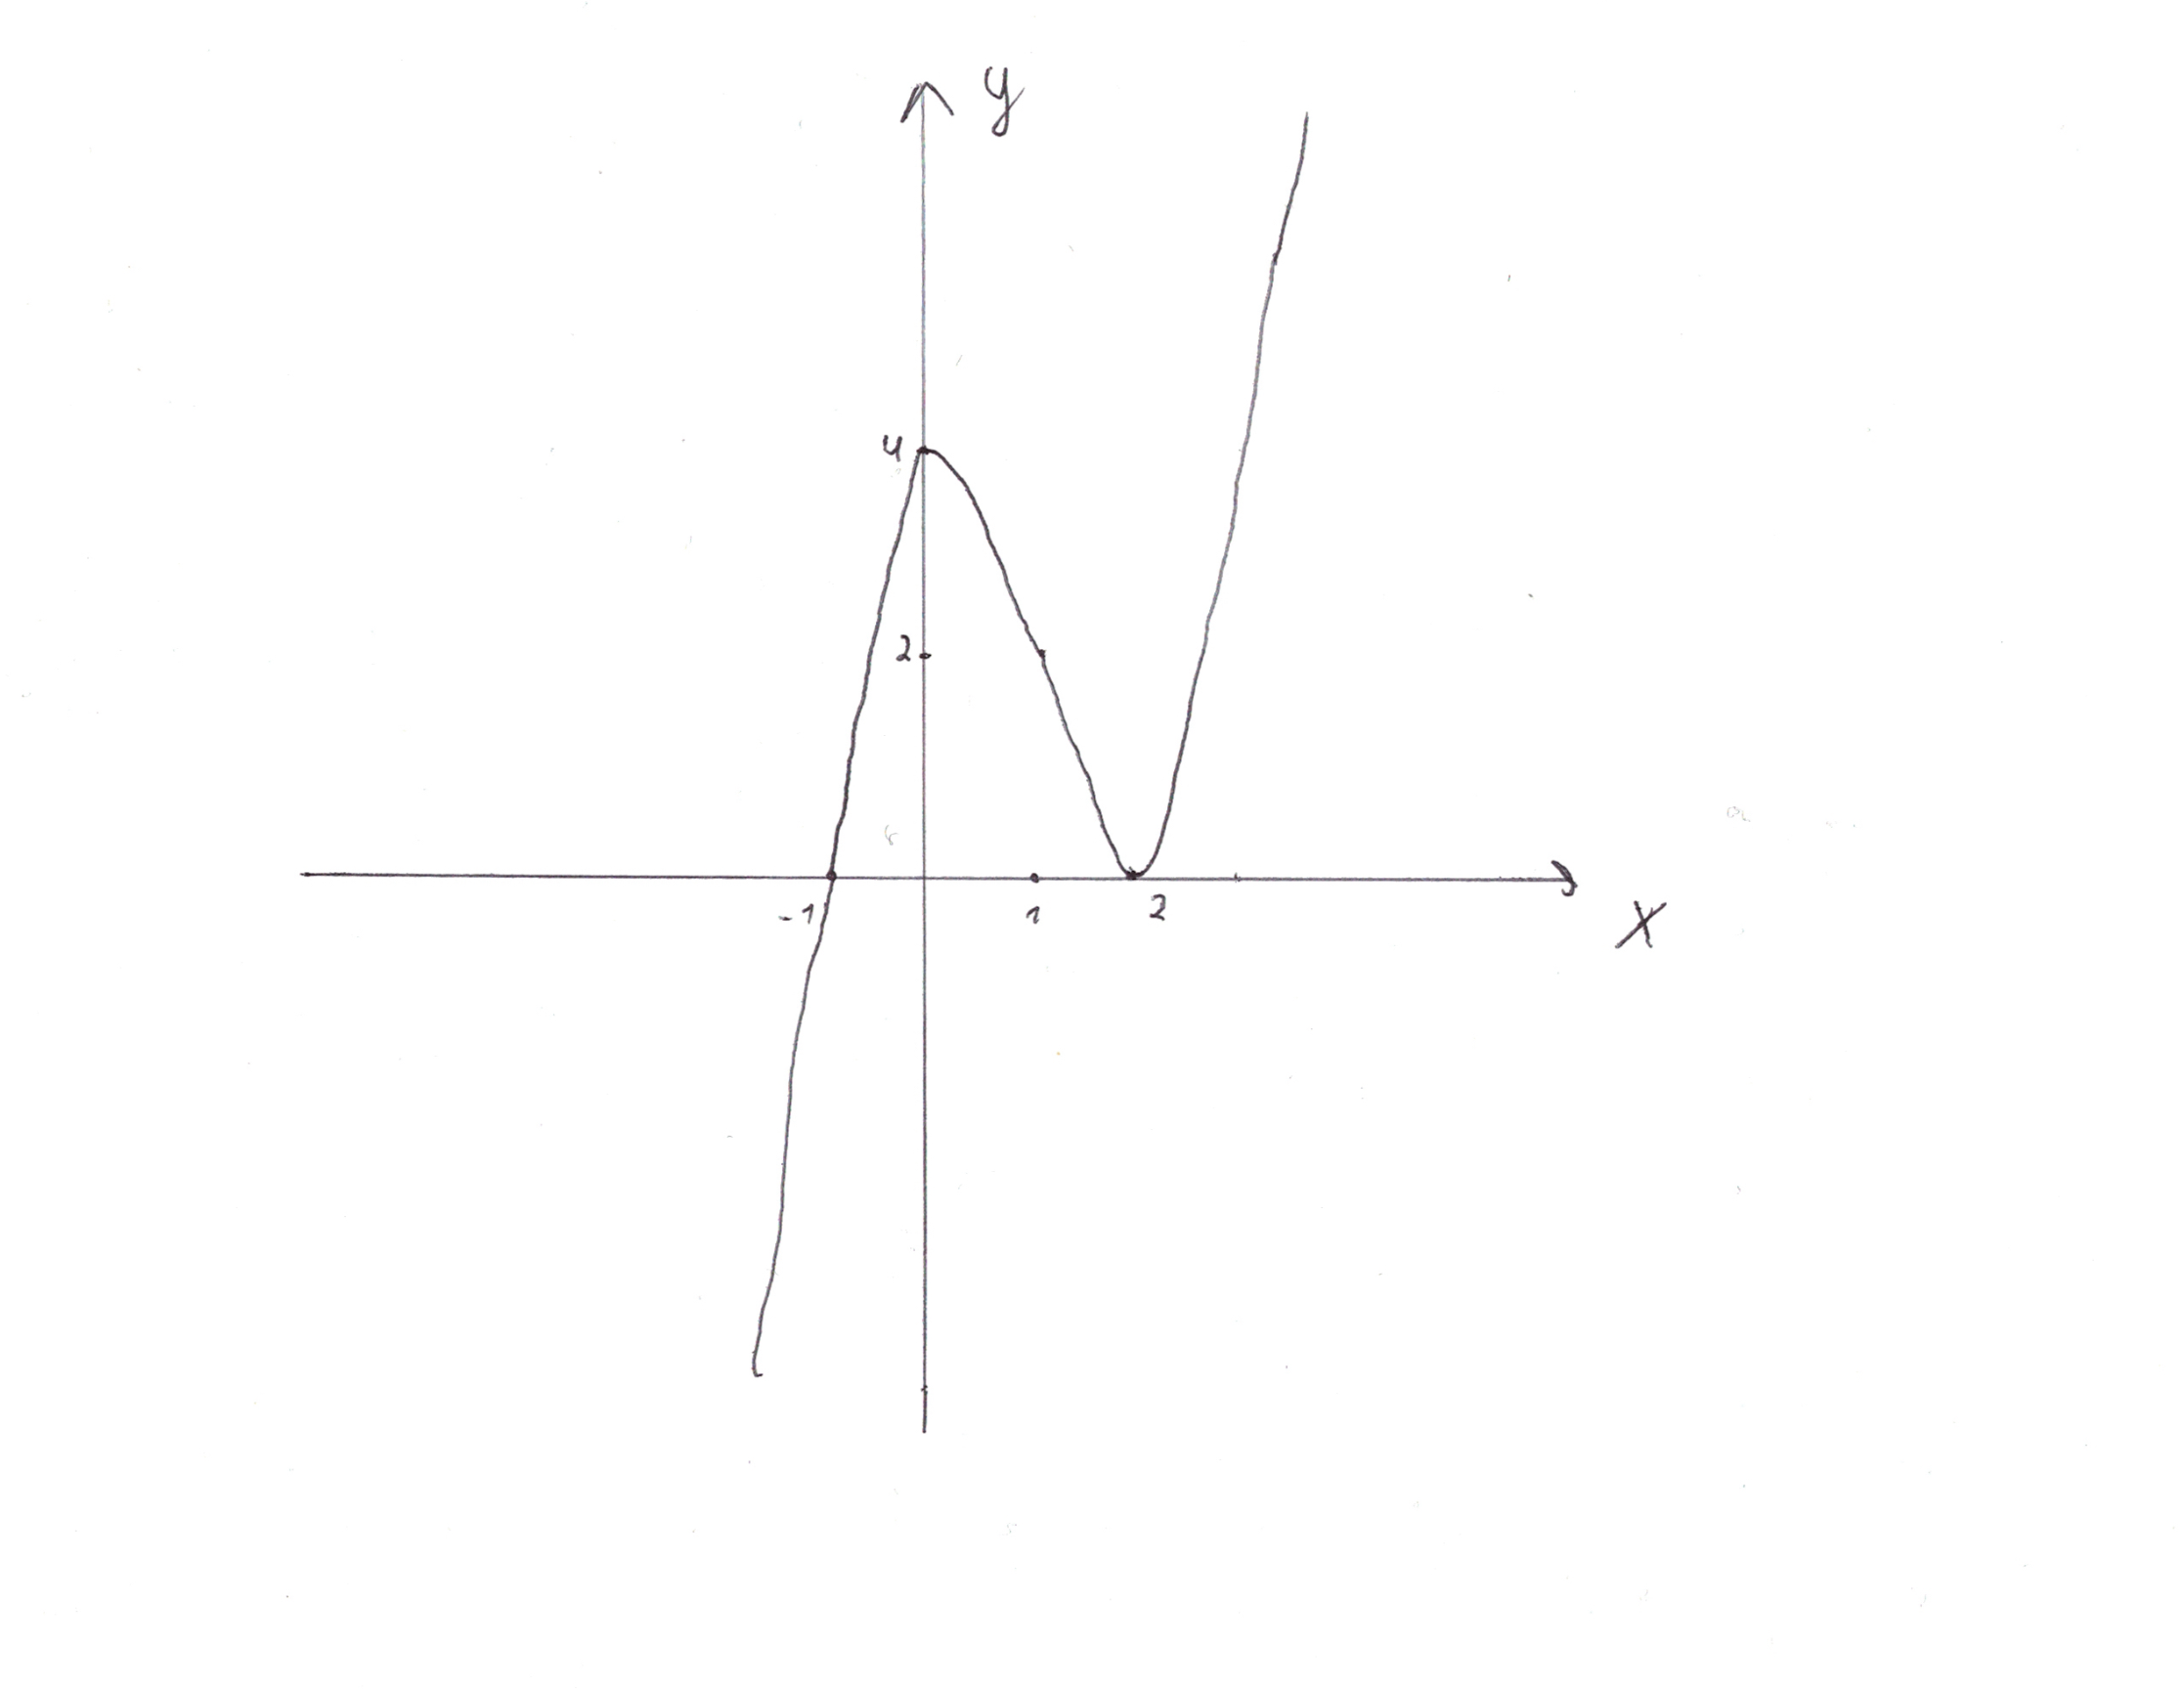
\includegraphics[scale=0.4]{grah1.png}
\end{center}
\end{enumerate}

\newpage
\subsection*{b)}
\[
f(x) = \frac{x^3(3x+4)}{(x+1)^3}
\]
Проведем исследование функции и построим её график.
\begin{enumerate}
\item \textbf{Область определения и поведение функции на границах:}

Функция неопределена в $x = -1$
\[
\lim_{x \rightarrow (-1)+} f(x) = \infty
\]
\[
\lim_{x \rightarrow (-1)-} f(x) = -\infty
\]
\[
\lim_{x \rightarrow \infty} f(x) = \infty
\]
\[
\lim_{x \rightarrow -\infty} f(x) = -\infty
\]

\item \textbf{Нули и знаки функции:}
\[
\frac{x^3(3x+4)}{(x+1)^3} = 0
\]
\[
x = 0; \;x = -\frac{4}{3}
\]
\item \textbf{Экстремумы и монотонность:}
\[
f'(x) = \frac{(3x^2(3x+4) + 3x^3)(x+1)^3 - x^3(3x+4)3(x+1)^2}{(x+1)^6} = 
\]
\[
= \frac{(12x^3 + 12x^2)(x+1) - 9x^4 - 12x^3}{(x+1)^4}  = \frac{3x^2(x+2)^2}{(x+1)^4}
\]
\[
f'(x) = 0 : \; x = -2; x = 0
\]
\[
f(-2) = -16; f(0) = 0
\]
\begin{center}
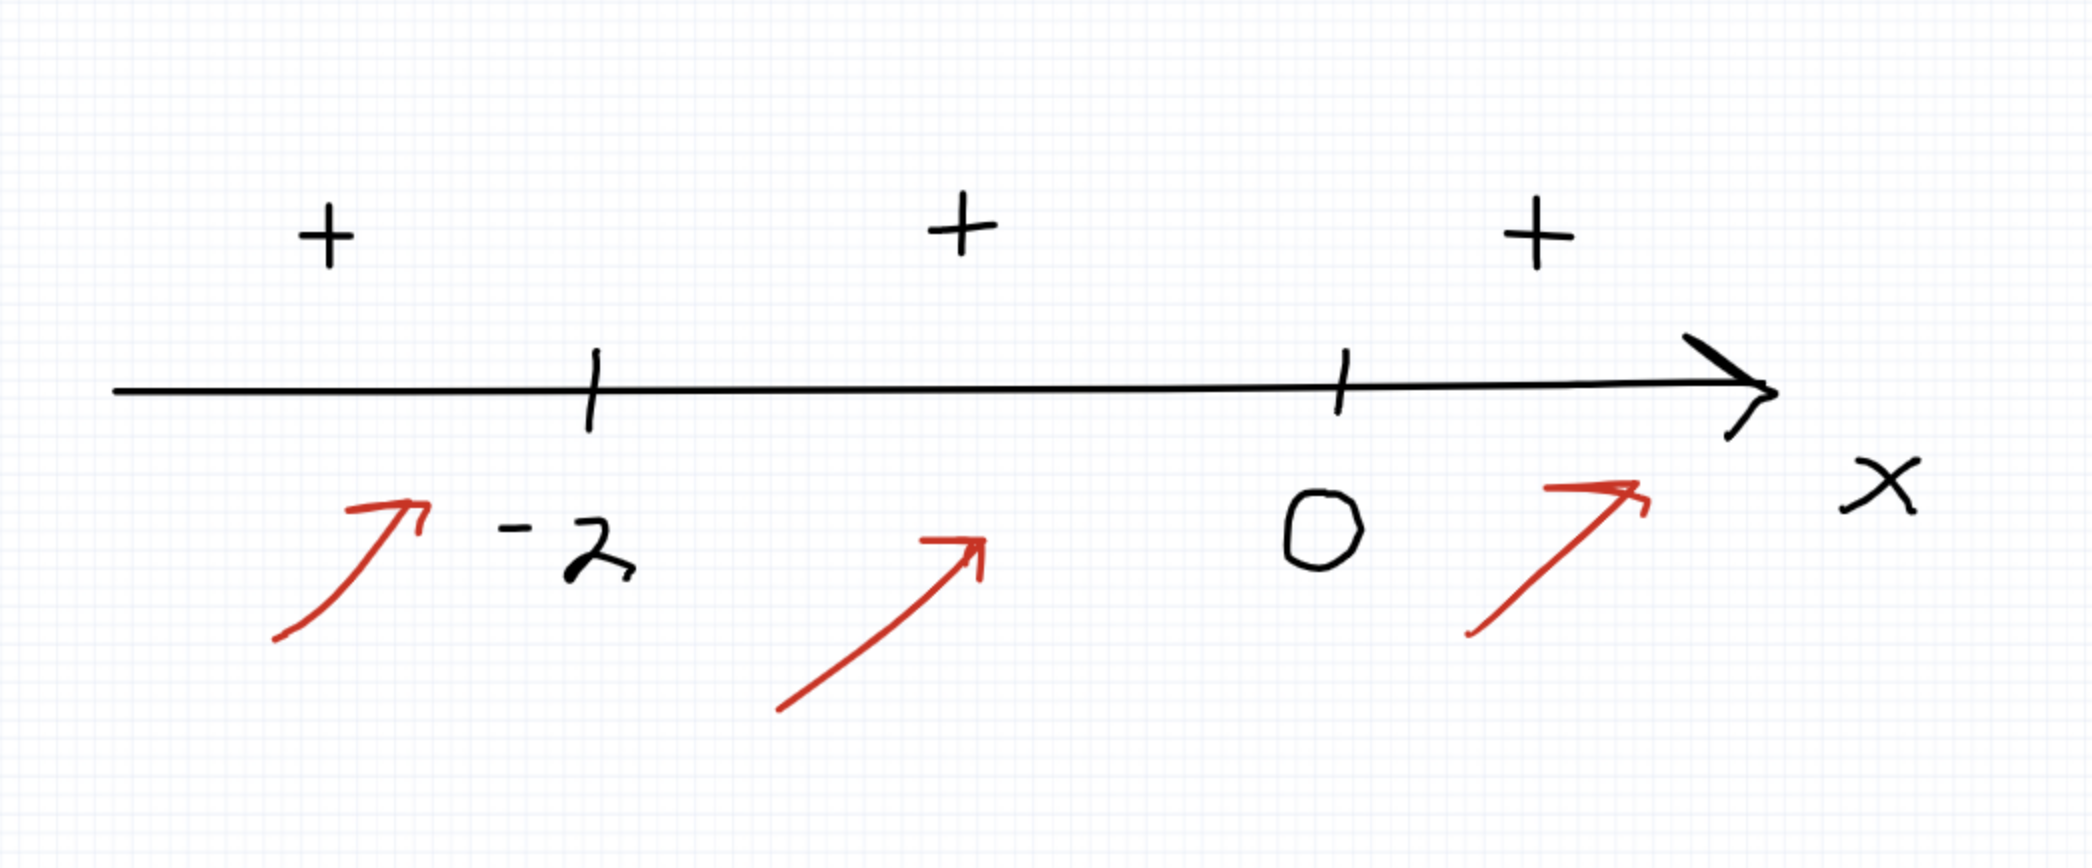
\includegraphics[scale=0.2]{3.png}
\end{center}
\item \textbf{Выпуклость:}
\[
f''(x) = \frac{(12x^3 + 36x^2 + 24x)(x+1)^4 - (3x^4 +12x^3 +12x^2)4(x+1)^3)}{(x+1)^8} = 
\]
\[
= \frac{12x^4 + 36x^3 + 24x^2 + 12x^5 + 36x^2 +24x -12x^4 -48x^5 -48x^2}{(x+1)^5} =
\]
\[
= \frac{12x^2+ 24x}{(x+1)^5} = \frac{12x(x+2)}{(x+1)^5}
\]
\[
f''(x) = 0 : \; x = 0; x = -2
\]
\begin{center}
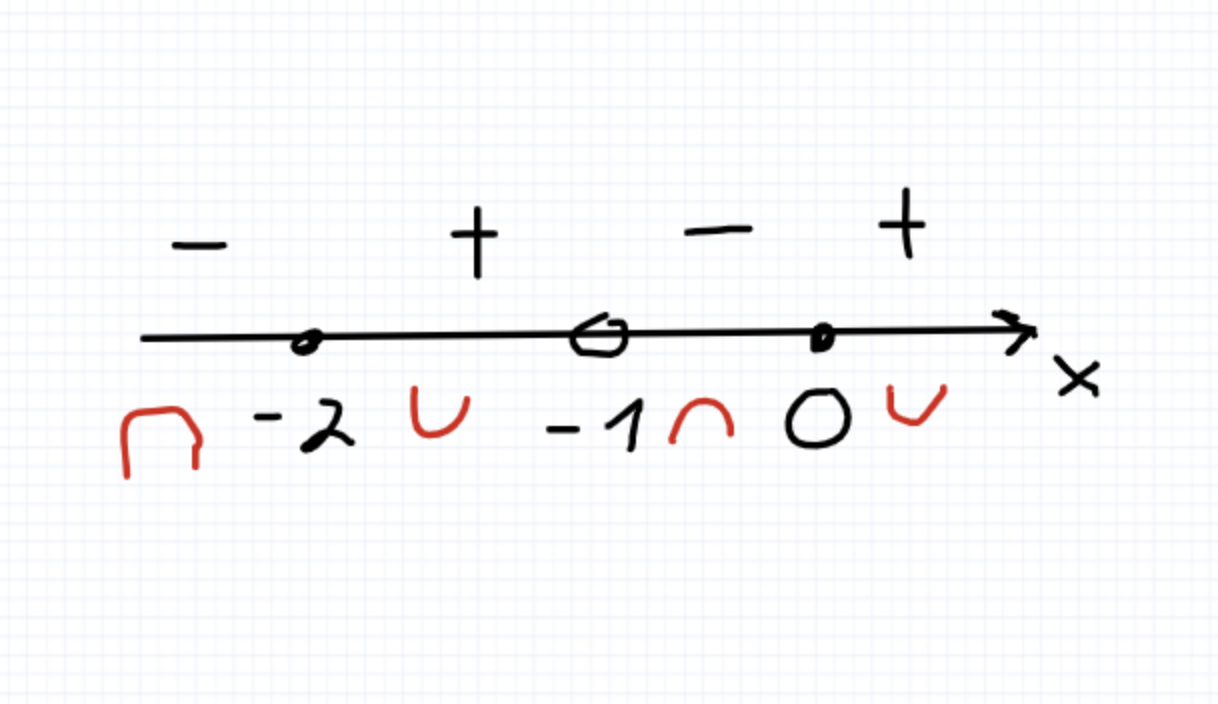
\includegraphics[scale=0.22]{4.png}
\end{center}
\item \textbf{Ассимптоты:}
\[
k = \lim_{x \rightarrow \infty} \frac{f(x)}{x} = \lim_{x \rightarrow \infty} \frac{x^3(3x+4)}{x(x+1)^3} = \lim_{x \rightarrow \infty} \frac{3x^4 + 4x^3}{x^4 + 3x^3 + 3x^2 + x} = \frac{3}{1} = 3
\]
\[
b = \lim_{x \rightarrow \infty}( f(x) - 3x) =\lim_{x \rightarrow \infty} (\frac{x^3(3x+4)}{(x+1)^3} -3x) = \lim_{x \rightarrow \infty} \frac{-5x^3 - 9x^2 -3x}{x^3 + 3x^2 +3x + 1 } = -5
\]
\[
y = 3x - 5
\]
Вертикальная ассимптота по точке разрыва $x = -1$
\item \textbf{График:}
\begin{center}
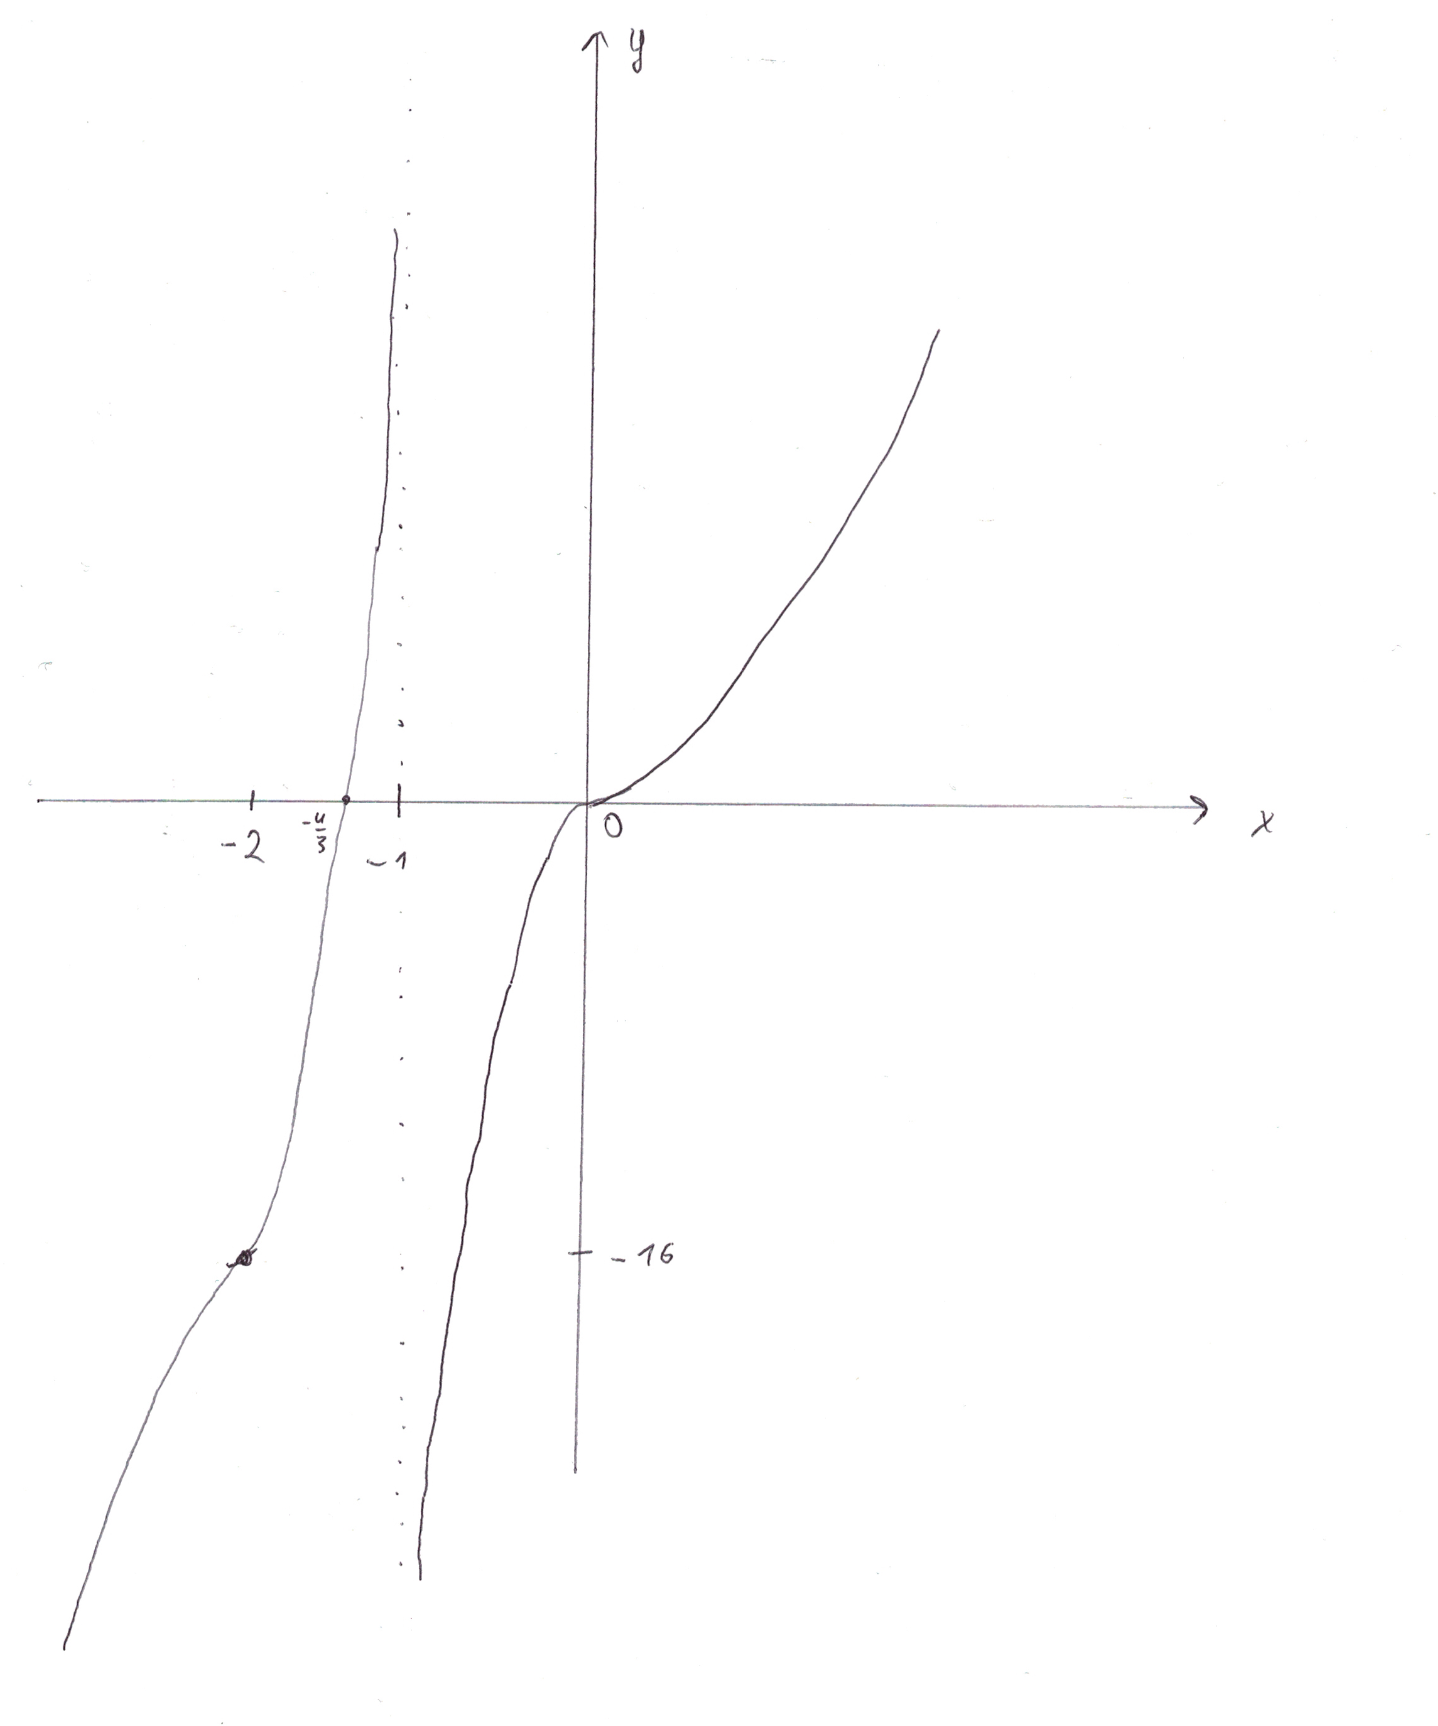
\includegraphics[scale=0.7]{grah2.png}
\end{center}
\end{enumerate}
\newpage
\subsection*{с)}
\[
f(x) = \sqrt{x} \cdot \ln x
\]
Проведем исследование функции и построим её график.
\begin{enumerate}
\item \textbf{Область определения и поведение функции на границах:}

$ x > 0$
\[
\lim_{x \rightarrow 0} \sqrt{x} \cdot \ln x =\lim_{x \rightarrow 0} \sqrt{x} \cdot (x-1) \cdot \frac{\ln (1 + (x-1))}{x-1} = \lim_{x \rightarrow 0} \sqrt{x} \cdot (x-1) \cdot 1 = 0 \cdot (-1) \cdot 1 = 0
\]
\[
\lim_{x \rightarrow \infty} f(x) = \infty
\]
\item \textbf{Нули и знаки функции:}
\[
\sqrt{x} \cdot \ln x = 0
\]
\[
x = 1
\]
\item \textbf{Экстремумы и монотонность:}
\[
f'(x) = \frac{\ln x}{2 \sqrt{x}} + \frac{\sqrt{x}}{x} = \frac{2 + \ln x}{2 \sqrt{x}}
\]
\[
f'(x) = 0 : x = \frac{1}{e^2}
\]
\[
f(\frac{1}{e^2}) = -\frac{2}{e}
\]
\begin{center}
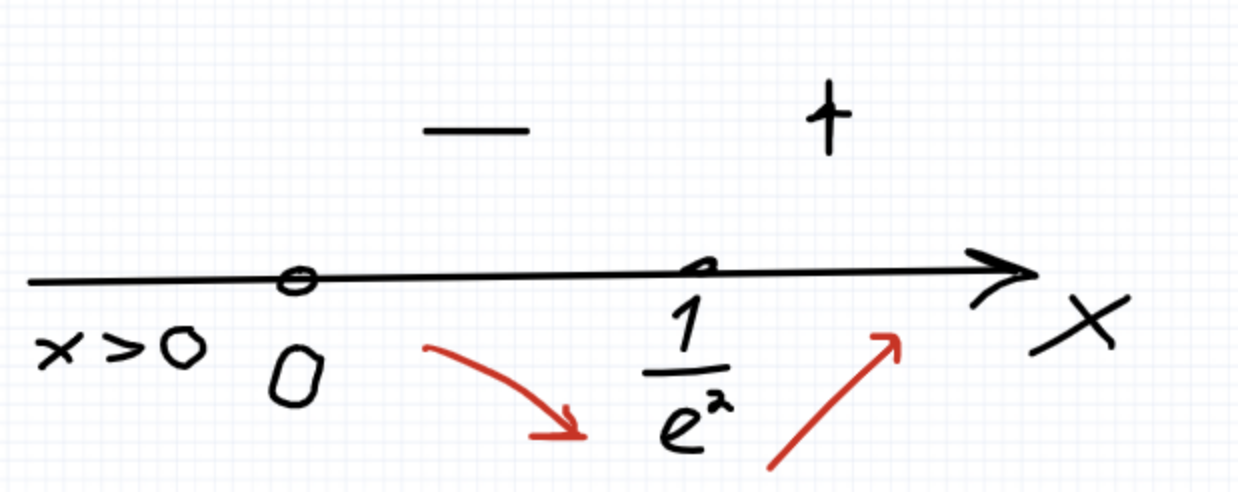
\includegraphics[scale=0.3]{5.png}
\end{center}
\item \textbf{Выпуклость:}
\[
f''(x) = \frac{\frac{2\sqrt{x}}{x} - \frac{2 + \ln x}{\sqrt{x}}}{4x} =  - \frac{\ln x}{4\sqrt{x} \cdot x}
\]
\[
f''(x) = 0 : \; x = 1
\]
\begin{center}
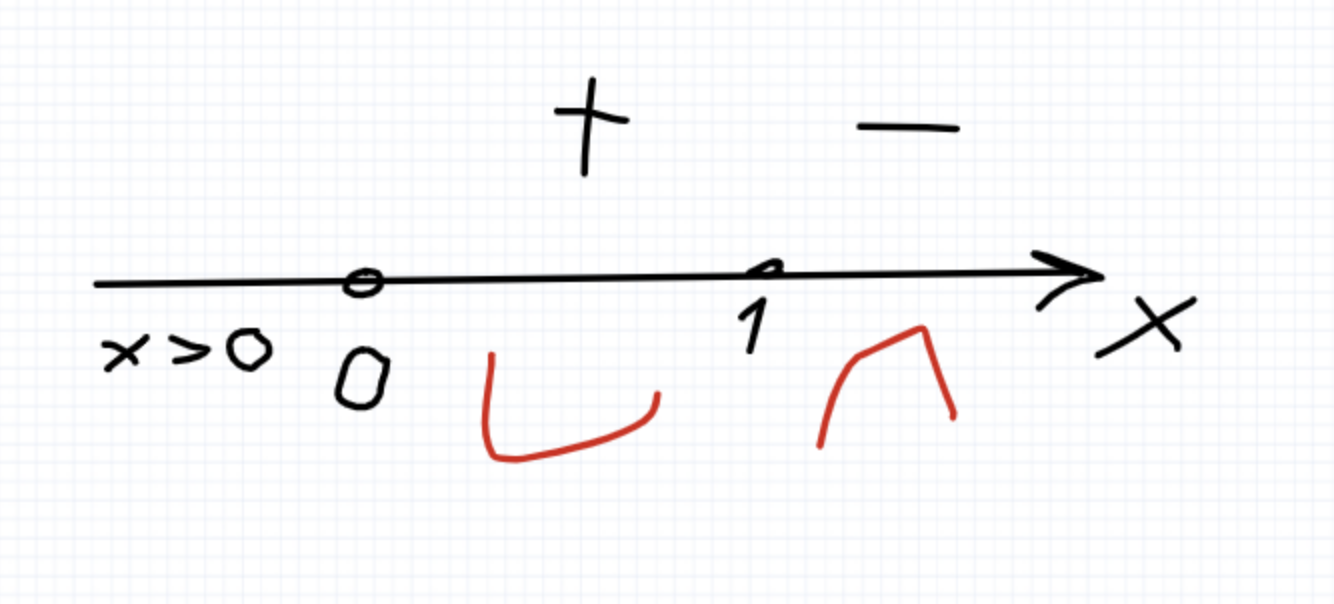
\includegraphics[scale=0.3]{6.png}
\end{center} 
\item \textbf{Ассимптоты:}
\[
k = \lim_{x \rightarrow \infty} \frac{\sqrt{x} \cdot \ln x}{x} = 0
\]
\[
b = \lim_{x \rightarrow \infty} (f(x) - 0x) = \infty
\]
\item \textbf{График:}
\begin{center}
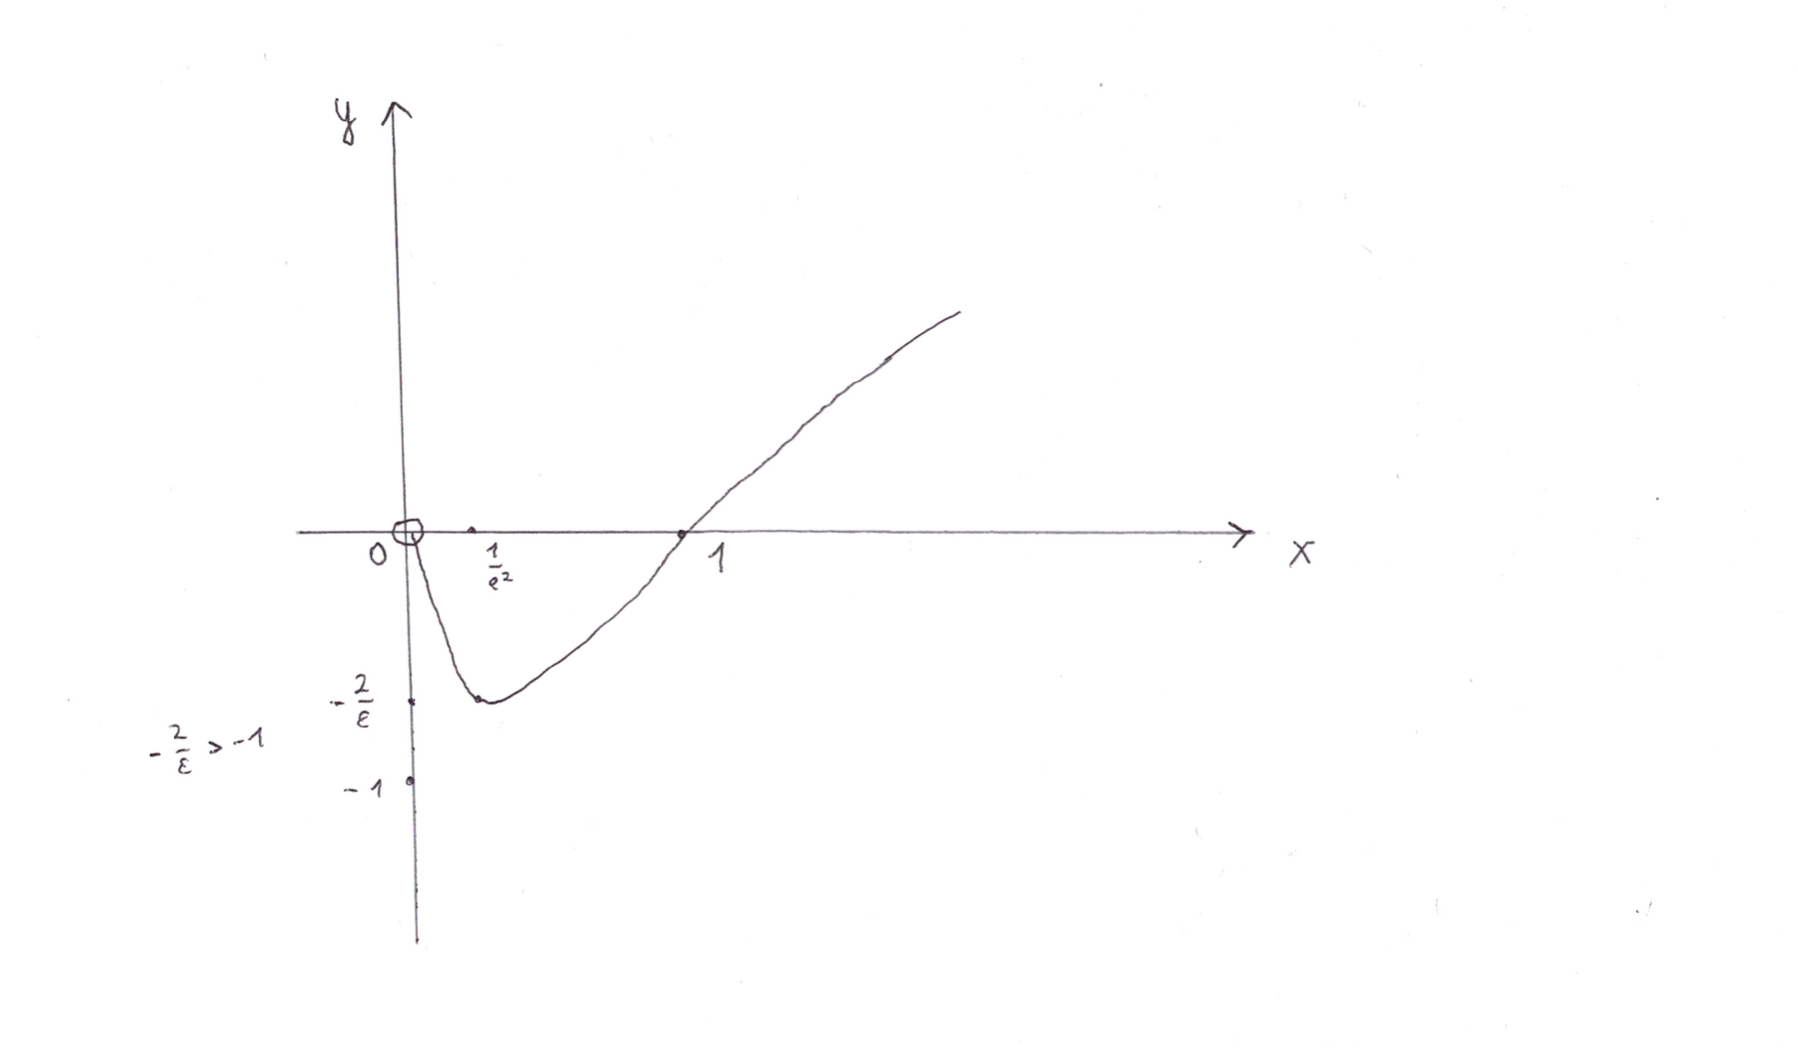
\includegraphics[scale=0.7]{grah3.png}
\end{center}
\end{enumerate}
\newpage
\subsection*{d)}
\[
f(x) = (x - 6) \cdot e^{-\frac{1}{x}}
\]
Проведем исследование функции и построим её график.
\begin{enumerate}
\item \textbf{Область определения и поведение функции на границах:}
 $ x \neq 0$
\[
(-\infty; 0) \cup (0; \infty);
\]
\[
\lim_{x \rightarrow -\infty} f(x) = -\infty
\]
\[
\lim_{x \rightarrow \infty} f(x) = \infty
\]
\[
\lim_{x \rightarrow 0+} f(x)= 0;
\]
\[
\lim_{x \rightarrow 0-} f(x) = -\infty
\]
\item \textbf{Нули и знаки функции:}
\[(x - 6) \cdot e^{-\frac{1}{x}} = 0
\]
\[
x = 6
\]
\item \textbf{Экстремумы и монотонность:}
\[
f'(x) = e^{-\frac{1}{x}} + (x-6) \cdot e^{-\frac{1}{x}} \cdot \frac{1}{x^2} = \frac{x^2 + x- 6}{e^{\frac{1}{x}} \cdot x^2}
\]
\[
f'(x) = 0; x^2 + x - 6 = 0; (x+3)(x-2) = 0
\]
\[
x = -3; x = 2
\]
\[
f(-3) = -9 \cdot e ^{\frac{1}{3}}; f(2) = -4 \cdot e^{-\frac{1}{2}}
\]
\begin{center}
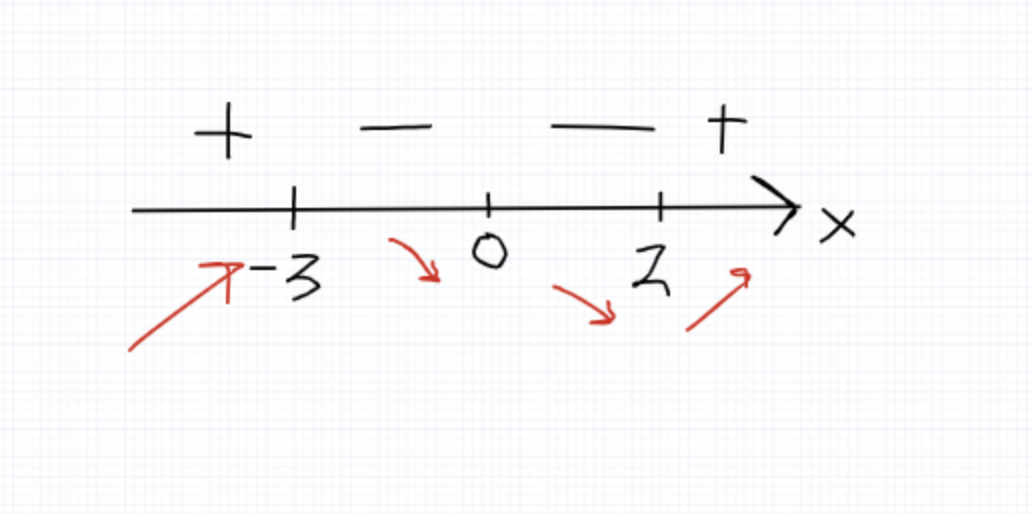
\includegraphics[scale=0.3]{7.png}
\end{center} 
\item \textbf{Выпуклость:}
\[
f''(x) = (2x+1) \cdot (e^{-\frac{1}{x}} \cdot x^{-2}) + \left(x^2 + x - 6\right) \cdot \left(e^{-\frac{1}{x}} \cdot \frac{x^{-2}}{x^2}  + e^{-\frac{1}{x}} \cdot \left(\frac{-2}{x^3}\right) \right) = 
\]
\[
=\frac{2x}{e^{1/x} \cdot x^2} + \frac{1}{e^{1/x} \cdot x^2} +  \frac{(x^2+x-6)}{e^{1/x} \cdot x^4} - \frac{2(x^2+x-6)}{e^{1/x} \cdot x^3} = 
\]
\[
= \frac{13x - 6}{x^4 \cdot e^{1/x}}
\]
\[
f''(x) = 0 : x = \frac{6}{13}
\]
\begin{center}
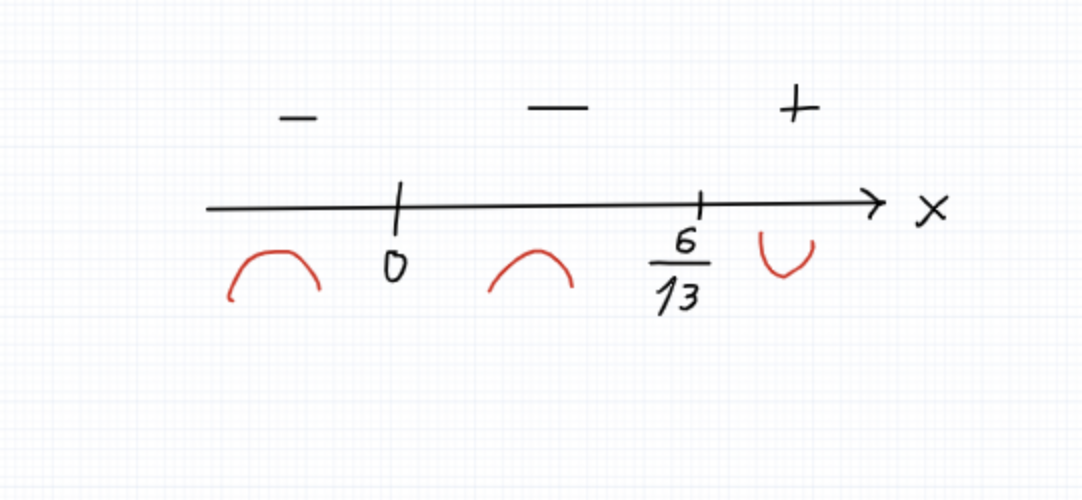
\includegraphics[scale=0.4]{8.png}
\end{center} 
\item \textbf{Ассимптоты:}
\[
k = \lim_{x \rightarrow \infty} \frac{x-6}{x \cdot e^{1/x}} = \lim_{x \rightarrow \infty} \frac{x-6}{x \cdot 1} = \lim_{x \rightarrow \infty} \frac{1 - \frac{6}{x}}{1} = 1
\]
\[
b = \lim_{x \rightarrow \infty} \left( \frac{x-6}{e^{1/x}} - 1 \cdot x \right) = \lim_{x \rightarrow \infty} \left(x -6 - x \cdot e^{1/x} \right) = -6 - \lim_{x \rightarrow \infty} \left(  x \cdot e^{1/x}  - x\right) = 
\]
\[
= - 6 - \lim_{x \rightarrow \infty} \frac{e^{1/x} -1}{\frac{1}{x}} \cdot \frac{x}{1} \cdot \frac{1}{x} = - 6- \lim_{x \rightarrow \infty}e^{1/x} = -6 -1 = -7
\]
\[
y = x - 7
\]
Вертикальная ассимптота в точке разрыва $ x = 0$
\item \textbf{График:}
\begin{center}
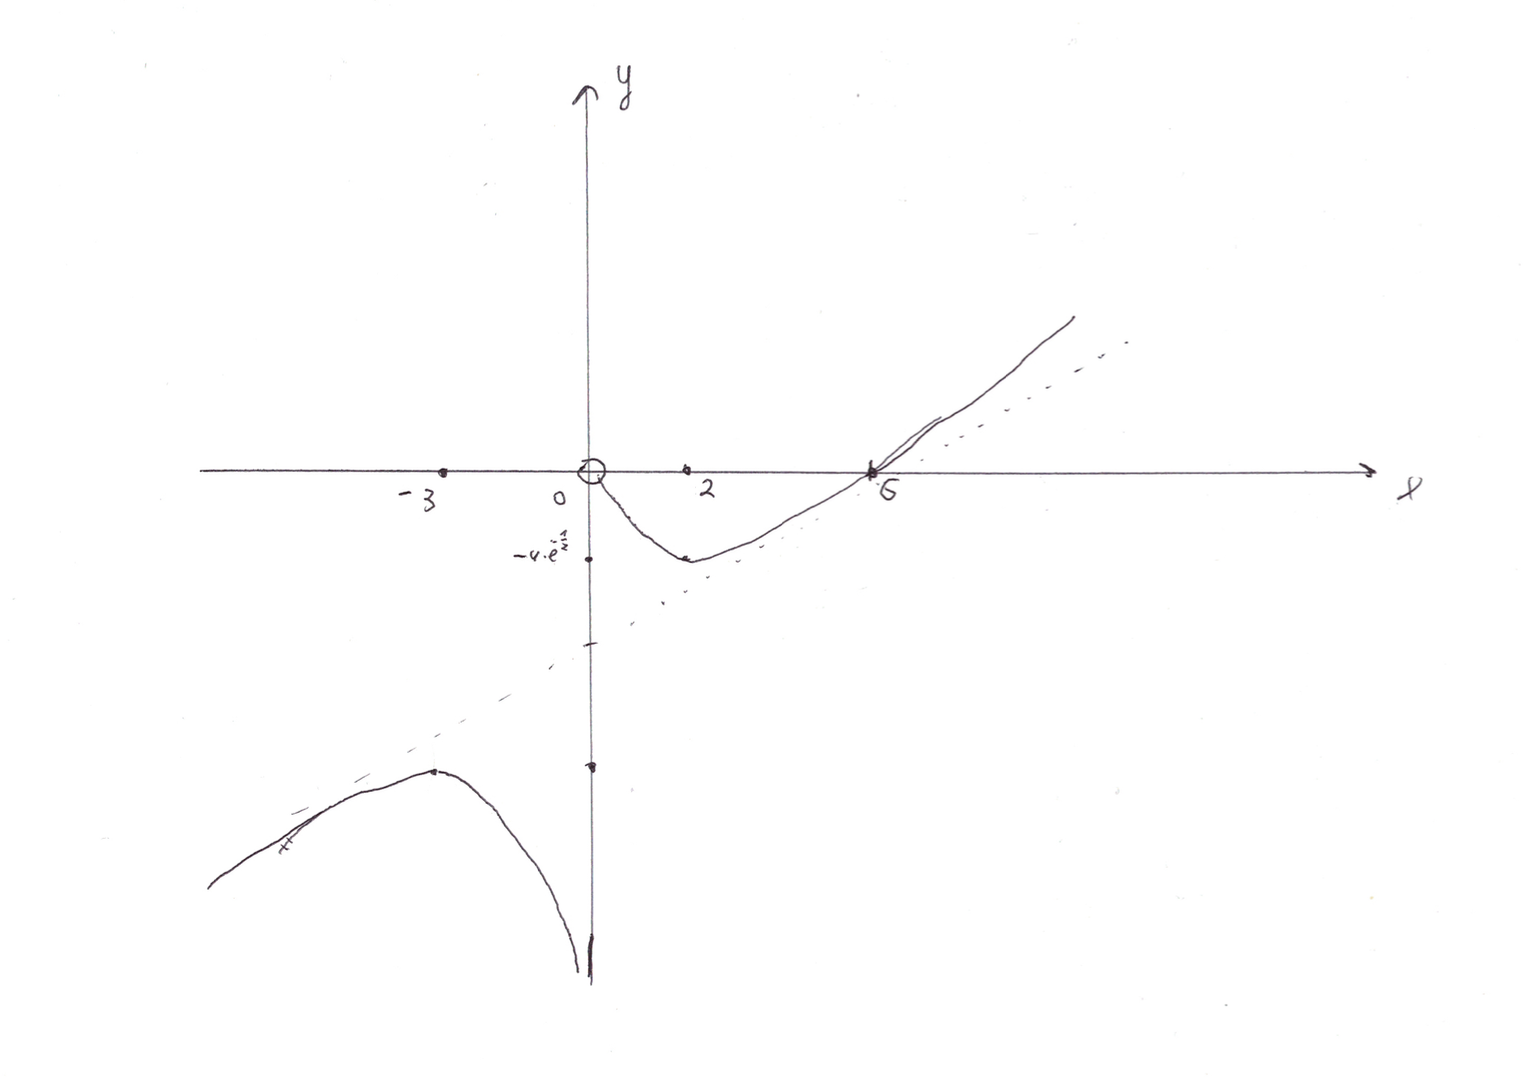
\includegraphics[scale=0.6]{grah4.png}
\end{center}
\end{enumerate}
\end{document}